\section{Триангуляция Делоне, связь с диаграммами Вороного. Алгоритм построения }

Триангуляция - максимальное планарное разбиение, к которому нельзя добавить ни одного ребра, соединяющего 2 вершины, без нарушения планарности. 

\textbf{Триангуляция Делоне} - триангуляция для заданного множества точек $S$, при котором для каждого $\Delta$-ка все точки из $S$, кроме вершин $\Delta$-ка лежат вне окружности, описанной вокруг этого треугольника. 
\begin{figure}[h!]
	\centering
	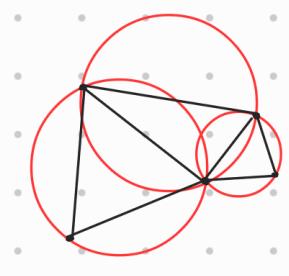
\includegraphics[width=0.4\linewidth]{img/14_1.png}
	\captionsetup{labelformat=empty}
	\caption{Триангуляция Делоне}
\end{figure}


\subsection*{Связь с диаграммой Вороного: }
\textbf{Теорема:} (двойственность диаграммы Вороного и триангуляции Делоне) 

Серединный перпендикуляр центров определяет ребро диаграммы Вороного $\Leftrightarrow$ точка на этом перпендикуляре, такая что: 
\begin{itemize}
	\item граница круга ($q$) содержит только центры $p_1$ и $p_2$ 
	\item внутренность круга не содержит других центров мн-ва $P$ 
\end{itemize}

\subsection*{Получение диаграммы Вороного из триангуляции Делоне }
\begin{figure}[h!]
	\centering
	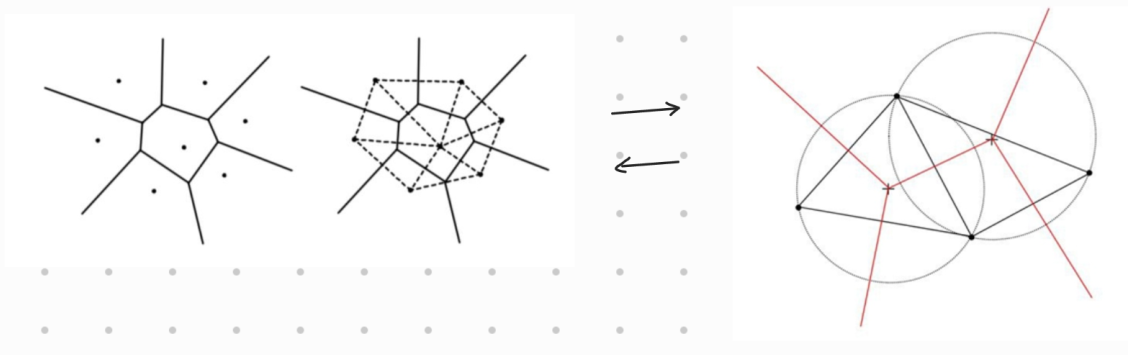
\includegraphics[width=0.5\linewidth]{img/14_2.png}
	\captionsetup{labelformat=empty}
	\caption{Диаграмма Вороного --- триангуляция Делоне}
\end{figure}


\subsection*{Алгоритм построения триангуляции Делоне:} 

\textbf{Наивный} 
\begin{enumerate}
	\item Перебираем все треугольники (все тройки точек из S) ($O(n^3)$) 
	\item Описываем вокруг каждого треугольника окружность $O(1)$ и проверяем, пуста ли каждая окружность. Те $\Delta$-ки, окружности которых являются пустыми, объявляются гранями триангуляции Делоне ($T$) - для одной $\Rightarrow$ ($T_i$) 
	\item Перебираем все пары выбранных $\Delta$-ов и проверяем на смежность $O(n^2)$ 
\end{enumerate}

\textbf{Итого:} $O(n^4)$ 

\subsection*{Триангуляция методом "разделяй и властвуй":} 
\begin{itemize}
	\item делим множество точек на мелкие множества (рекурсивно) 
	\item затем объединять оптимальные триангуляции 
\end{itemize}

\textbf{"удаляй и строй": объединение 2-х триангуляций} 
\begin{enumerate}
	\item Ищем 2 общие касательные (верхняя и нижняя). \\
	Верхнюю обозначаем за базовую линию. 
	\item Ищем внешний узел, ближайший к базовой линии \\
	и строим треугольник по базовой линии и этому узлу. 
	\item Берём новую сторону $\Delta$-ка за базовую линию, повторяем процесс до нижней касательной. 
\end{enumerate}

\begin{figure}[h!]
	\centering
	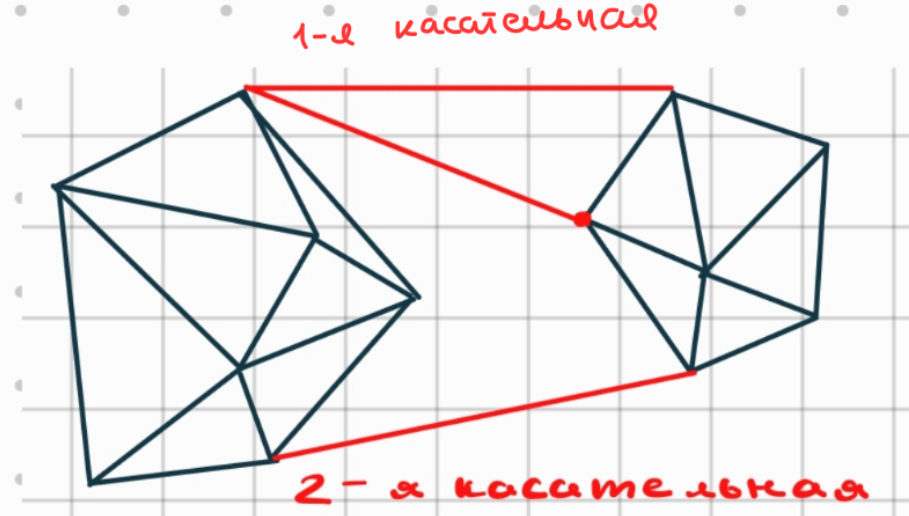
\includegraphics[width=0.4\linewidth]{img/14_3.png}
	\captionsetup{labelformat=empty}
	\caption{}
\end{figure}

или 

\textbf{"строй и перестраивай"} 
\begin{enumerate}
	\item Ищем 2 общие касательные (верхняя и нижняя).
	Верхнюю обозначаем за базовую линию. 
	\item Рассматриваем 2 ближайшие к базовой прямой точки 
	строим 2 $\Delta$-ка 
	\item Выбираем тот треугольник, min угол которого больше 
	($\Rightarrow$ этот треугольник более равносторонний и будет перестроен с меньшей вероятностью) 
	\item Берём новую сторону $\Delta$-ка за базовую линию, повторяем процесс до 2-й касательной. 
	\item Проверка всех $\Delta$-ов на условие Делоне. 
\end{enumerate}

\begin{figure}[h!]
	\centering
	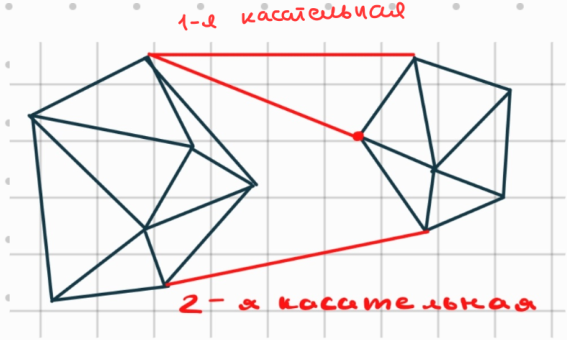
\includegraphics[width=0.4\linewidth]{img/14_4.png}
	\captionsetup{labelformat=empty}
	\caption{}
\end{figure}

\subsection*{Сложность алгоритма:} 
\begin{itemize}
	\item разбиение множества точек $O(\log n)$ 
	\item каждое объединение $O(n)$ 
\end{itemize}
\textbf{Всего:} $O(n \log n)$